\section{Introduzione}
\label{introduzine}
Per il progetto del corso di Informatica e Programmazione si è scelto di realizzare un robot mobile con azionamento differenziale a due ruote con componenti \emph{Makeblock}.

\subsection{Hardware}
Non avendo vincoli progettuali si è scelto di utilizzare un struttura semplice come riportata in figura \ref{}. %inserire riferimento figure.
La parte elettronica è basata sulla scheda MeOrion baseboard, un modulo a ultra suoni per il rilevamento degli ostacoli, due moduli per i sensori tipo MeLineFollower, un modulo bluetooth, in figura \ref{schema}, il dettaglio dei collegamenti. La lista completa dei componenti in tabella \ref{bom}.
La scelta di adottare una coppia di sensori di linea è stata vagliata per una migliore lettura del percorso, identificazione di casi particolari come ad esempio curve a 90$^{\circ}$, incroci e per un miglior controllo dei motori.

\begin{figure}[htp]
\centering
\hfill
\begin{minipage}[b]{.65\columnwidth}
 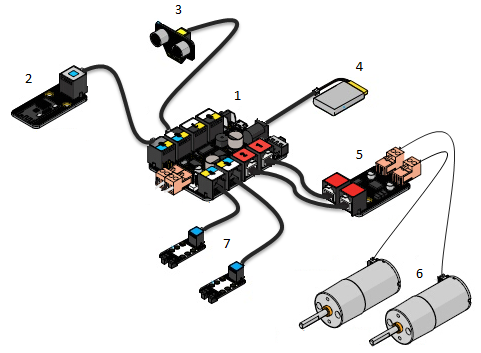
\includegraphics[width=0.75 \textwidth]{SCHEMA}
	\caption{Schema di collegamento}
	\label{schema}
\end{minipage}
\begin{minipage}[b]{.3\columnwidth}
  \begin{tabular}{ccl}
	Num. & Q.ta & Modulo\\
	\hline
	1		&		1	&	MeOrion\\
	2		&		1	&	MeBluetooth \\
	3		&		1	&	MeUltra \\
	4		&		1	&	Batteria Li-Po\\
	5		&		1	&	Me\\
	6		&		2	&	MeDCMotor\\
	7		&		2	&	MeLineFollower	\\
	\hline
  \end{tabular}
  \captionof{table}{Lista componenti}
  \label{bom}
\end{minipage}\hspace*{\fill}
\end{figure}

\subsection{Software}
Il software che gestisce la logica del è stato pensato modulare per aumentare la facilità di realizzazione e manutenzione.
Si articola su tre \emph{layer} le librerie proprietarie Makeblock uililizzate per gestire i moduli collegati alle porte della scheda, una classe che implementa la macchina a stati finiti che gestisce gli stati dell'automa infine una classe che connette i due livelli precedenti permettendo la lettura degli input dai sensori e il verificarsi delle condizioni per passare da uno stato all'altro.